\documentclass[a5paper,pagesize,10pt,bibtotoc,pointlessnumbers, normalheadings,DIV=9,twoside=false]{scrbook}

% twoside, openright
\KOMAoptions{DIV=last}

\usepackage{trajan}
 
\usepackage[ngerman]{babel}
\usepackage[utf8]{inputenc}
\usepackage[T1]{fontenc}

\usepackage[babel,german=guillemets]{csquotes}

\usepackage[sc]{mathpazo}
\linespread{1.05} 

\usepackage{verbatim} % for comments
\usepackage{listings} % for comments

%\setlength{\parindent}{10pt}
%\setlength{\parskip}{1.4ex plus 0.35ex minus 0.3ex}
%\setlength{\parskip}{1.4ex plus 0.35ex minus 0.3ex}

\usepackage{blindtext}
\newcommand{\q}[1]{>>\textit{#1}<<}

\usepackage{graphicx}

\title{Memory}   
\author{J.Y.} 
\date{\today} 

\begin{document}


%=========================================
\begin{titlepage}
		\centering{
			{\fontsize{40}{48}\selectfont 
			Memory}
		}\\
			
		\vspace{10mm}
		\centering{\Large{J.Y.}}\\
		\vspace{\fill}
		\centering \large{2021}
\end{titlepage}


%=========================================
\newpage{}
\thispagestyle {empty}

\vspace*{2cm}

\begin{center}
	\Large{\parbox{10cm}{
		\begin{raggedright}
		{\Large 
			\textit{Do what you think is interesting, 
			do something that you think is fun and worthwhile, 
			because otherwise you won’t do it well anyway.}
		}
	
		\vspace{.5cm}\hfill{---Brian W. Kernighan}
		\end{raggedright} 
	}
}
\end{center}

\newpage


%=========================================
%\blinddocument

\section{Memory Layout}
A typical memory representation of a C program consists of the following sections.
\begin{enumerate}
	\item Text segment
	\item Initialized data segment
	\item Uninitialized data segment
	\item Stack
	\item Heap
\end{enumerate}

\begin{figure}[!htb]
	\centering
	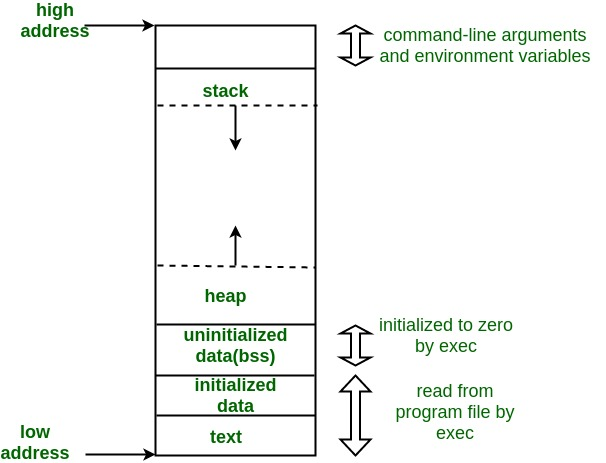
\includegraphics[width=\textwidth]{pictures/memoryLayoutC.jpg}
\end{figure}

\subsection{Text segment}
A \textbf{text segment}, also known as a \textbf{code segment} or simpley as \textbf{text},
is one of the sections of a program in an object file or in memory,
which contains executatble instructions.

As a memory region, a text segment may be place below the heap or stack 
in order to prevent heaps or stack overflows from overwriting it.

Usually, the text segment is sharable so that only a single copy needs to be 
in memory for frequently executed programs, such as text editors, the C compiler, 
the shells, and so on. Also the text segment is often read-only, to prevent program
from accidently modifying its instructions.


\subsection{Initialized Data Segment}
\textbf{Initialized data segment}, usually called simply the data segment. 
A data segment is a portion of the virtual address space of a program, 
which contains the global variables and static variables that are initialized by the programmer.

Note that, the data segment is not read only, since the values of the variables can be altered 
at run time.

This segment can be further classified into the initialized read-only and the initialized
read-write area.
For instance, the global string defined by char s[] = "Hello World" in C, and a C statement like 
int debug = 1 outside the main would be stored in the initialized read-write area.
And a global C statement like const char* str = "Hello World" makes the string literal "Hello World" 
to be stored in the initialized read-only area, and the pointer variable in the initialized 
read-write area.  

\subsection{Uninitialized Data Segment}
Uninitialized data segement often called the "bss" segment, named after an ancient assembler operator 
that stood for "block stated by symbol". 
Dta in this segement is initialized by the kernel to arithmetic 0 before the program starts executing.
Uninitialized data stats at the end of the data segment and contains all global varibales and static 
variables that are initialized to zero or do not have explicit initialization in source code.
For instance, a variable declared static in i, or a global variable declared int j.


\subsection{Stack}
The stack area tradidtionally adjoined the heap area and grew in the opposite direction; 
when the stack pointer met the heap pointer, free memory was exhausted.

The stack area contains the program stack, a LIFO structure, typically located in the higher parts of memory.
A stack pointer register tracks the top of the stack; it is adjusted each time a value is 
pushed onto the stack. 
The set of values pushed for one function call is termed a "stack frame"; a stack frame consists 
at minimum of a return address.

Stack, where automatic variables are stored, along with information that is saved each time a function 
is called.
Each time a function is called, the address of where to return to and certain information about 
the caller's environment, such as some of the machine registers, are saved on the stack. 
The newly called function then allocates room on the stack for its automatic and temporary 
variables. 
This is how recursive functions in C can work. 
Each time a recursive function calls itself, a new stack frame is used, so one set of variables 
doesn't interfere with the variables from another instance of the function.


\subsection{Heap}
Heap is the segment where dynamic memory allocations usually takes place.
The heap area begins at the end of the BSS segment and grows to larger addresses from there. 
The heap area is managed by malloc, realloc, and free, which may use the brk and sbrk system calls 
to adjust the size.

Note that the use of brk/sbrk and a single "heap area" is not required to fulfill the contract of 
malloc/realloc/free; they may also be implemented using mmap to reserve potentially non-contiguous 
regions of virtual memory into the process' virtual address space.

The heap area is shared by all shared libraries and dynamically loaded modules in a process. 



%=========================================
\begin{comment}
Just some notes, not visible in pdf.
\end{comment}


\end{document}

